\chapter{Test e risultati}

In questa sezione verranno descritti i diversi test condotti. Dopo una breve introduzione che presenta il lavoro svolto, seguirà una parte dedicata ai grafici dei risultati ottenuti, accompagnata da analisi e considerazioni pertinenti. Infine, saranno presentate le conclusioni finali.

I valori ottenuti, non riportati qui per ovvie ragioni, possono essere trovati in un \textit{repository Github} apposito \cite{ACPlot}.

\section{Flussi TCP con e senza QoS}
Si vuole simulare un ambiente in cui un nodo, facente le funzioni di server, vuole trasmettere un flusso di pacchetti verso un altro nodo che agirà come un client. 
Nei casi di test che successivamente saranno analizzati, i quattro dispositivi Rock che compongono il testbed verranno suddivisi in due gruppi separati, due in uno e i restanti due in un altro, ognuno con una funzione specifica.

I due gruppi saranno:
\begin{itemize}
    \item \textit{Gruppo Cx}: esso sarà composto da due dispositivi che simuleranno, con modalità che verranno discusse a breve, un ambiente in cui sono presenti uno svariato numero di veicoli che porteranno il canale di trasmissione a congestionarsi, in maniera completa o parziale.
    \item \textit{Gruppo Tx}: esso, invece, sarà composto da due dispositivi che comunicheranno mediante due flussi TCP in parallelo mediante l'utilizzo del comando iPerf. Uno di essi agirà come client, che andrà a connettersi e a scaricare delle informazioni dall'altro che fungerà da server.
\end{itemize}

\begin{figure}[h!]
    \centering
    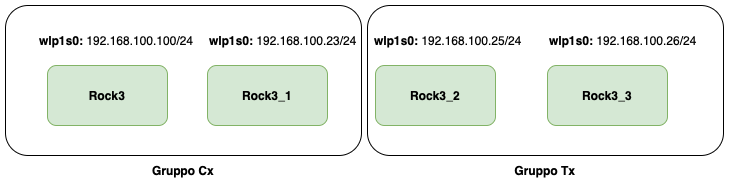
\includegraphics[width=1\textwidth]{diagramma_test.png}
    \caption{Diagramma dispositivi Rock}
    \label{fig:diagramma}
\end{figure}

Sono previsti tre principali casi di test:

\begin{itemize}
    \item \textit{Congestione nulla}: assenza di \textit{QoS} nei flussi dei dispositivi del \textit{Gruppo Tx} e assenza di congestione del canale, quindi il \textit{Gruppo Cx} sarà spento.
    \item \textit{Congestione parziale}: assenza di \textit{QoS} nei flussi dei dispositivi del \textit{Gruppo Tx} e parziale congestione del canale, attuata mediante l'invio in broadcast di CAM da ognuno dei due dispositivi facenti parte del \textit{Gruppo Cx} ogni 5 ms.
    \item \textit{Congestione massima}: assenza di \textit{QoS} nei flussi dei dispositivi del \textit{Gruppo Tx} e totale congestione del canale, attuata mediante trasmissione UDP in \textit{flooding} in broadcast da parte di ognuno dei due dispositivi del \textit{Gruppo Cx}.
\end{itemize}

Questi stessi casi verranno, inoltre, ripetuti andando ad applicare delle politiche di \textit{QoS}: un flusso (\textbf{Stream ID 1}) verrà assegnato alla categoria con priorità maggiore, ovvero \textit{Access Category Voice} (AC\_VO), mentre l'altro (\textbf{Stream ID 2}) alla categoria minore, ovvero \textit{Access Category Background} (AC\_BK).

Per fare ciò, verrà sempre utilizzato il comando iPerf, già precedentemente discusso, con i dovuti parametri. Nella fattispecie:

\begin{itemize}
    \item \textit{Rock Server}: \verb|iperf -s -i 1 -w 416K -y C -o output.csv|.
    \item \textit{Rock Client - flusso 1}: \\\verb|iperf -c 192.168.100.xxx -t 30 -b 10m -A VO| per il flusso a priorità maggiore.
    \item \textit{Rock Client - flusso 2}: \\\verb|iperf -c 192.168.100.xxx -t 30 -b 10m -A BK| per il flusso a priorità minore.
\end{itemize}

I due comandi sul client sono stati lanciati contemporaneamente dalla stessa \textit{command line} mediante l'utilizzo dell'operatore \textit{\&}; per ragioni di comodità riguardo la raccolta dei dati, in modo che il primo processo iPerf a partire fosse quello con priorità \textit{VO}, si è usato un artificio del genere:

\verb|iperf xxx -A VO & sleep 0.05 && iperf xxx -A BK| \\
\noindent Questo perchè il primo iPerf, anche se lanciato in principio, può non essere loggato come \textit{Stream ID 1} dal dispositivo server, per ovvie ragioni di scheduling dei processi e per via dell'\textit{handshaking} TCP; l'uso del comando \textit{sleep}, anche se ad effetto trascurabile per gli scopi in analisi, evita ciò.

L'indirizzo IP usato nei due comandi è relativo a quello appartenente all'interfaccia \textit{wlp1s0} del dispositivo facente funzione di server.

La velocità massima teorica di trasmissione del canale è fissata a 10 Mbps (lo si può notare dal parametro \verb|-b 10m| del comando iPerf).

Nei casi senza politiche di \textit{QoS} sono stati utilizzati i medesimi comandi, senza ovviamente il parametro \verb|-A| che delinea le varie priorità.

Per quanto concerne il raggiungimento di un eventuale congestione del canale, essa è stata raggiunta nei seguenti modi:

\begin{itemize}
    \item \textit{Caso senza congestione}: i dispositivi appartenenti al \textit{Gruppo Cx} non trasmettono alcunchè.
    \item \textit{Caso con congestione parziale}: i dispositivi appartenenti al \textit{Gruppo Cx}, come già detto poc'anzi, trasmettono ognuno un singolo pacchetto CAM ogni 5 ms; per tale scopo è stato lanciato sia su uno che sull'altro Rock lo script riportato in \autoref{udp_packets} con, come parametri, un \textit{message\_size} pari a 256 byte e lo \textit{sleep\_time} pari a 0.005; è stata scelto questo intervallo di tempo in quanto, tenendo conto che in caso di veicolo fermo esso invierebbe un CAM ogni 1 secondo, viene simulato un ambiente con 200 veicoli presenti.
    \item \textit{Caso con congestione totale}: i dispositivi appartenenti al \textit{Gruppo Cx} fanno flooding UDP mediante l'esecuzione del comando \verb|iperf -u -c 192.168.100.xxx| \verb| -t 300 -b 10m|; in questo caso si vuole simulare un ambiente con un numero veramente elevato di veicoli e molto maggiore del caso precedente.
\end{itemize}

In quest'ultimo caso, a causa delle limitazioni architetturali di iPerf, non è stato possibile inviare pacchetti UDP in broadcast. Poiché solo due dispositivi sono incaricati di effettuare flooding, la congestione viene raggiunta trasmettendo messaggi UDP da un dispositivo del \textit{Gruppo Cx} all'altro in unicast, specificando come parametro per iPerf l'indirizzo IP dell'interfaccia \textit{wlp1s0} del Rock destinatario.

La scelta del protocollo UDP per effettuare \textit{flooding}, anzichè il TCP, è stata effettuata per ovvie ragioni: mancanza di politiche riguardanti il controllo di flusso, perdita dei pacchetti e controllo sull'ordine di ricezione di quest'ultimi. Inoltre, l'invio di essi con una dimensione inferiore a 2346 byte (iPerf, di default, invia pacchetti UDP di soli 1470 byte a differenza del TCP che hanno una dimensione pari a 8 KB \cite{iperf}), consente alle interfacce Wireless di poter trasmettere i vari frame senza attuare il meccanismo di RTS/CTS.

In conclusione, per ogni simulazione sono state effettuati 5 \textit{run} distinti, ciascuno della durata di 30 secondi. Questa scelta è stata fatta per ottenere risultati il più affidabili possibile, permettendoci di escludere la parte iniziale dell'handshake del protocollo TCP, che potrebbe influenzare i valori iniziali in modo non desiderato.

Verranno, ora, mostrati i risultati ottenuti mediante dei grafici per ogni singolo caso di studio:

\begin{itemize}
    \item il primo mostrerà l'andamento del throughput medio nel corso della simulazione;
    \item il secondo consisterà nel \textit{plot} del throughput di ogni singola \textit{run};
    \item il terzo visualizzerà il carico del canale per tutta la durata della simulazione, inclusi alcuni istanti prima e dopo in modo da mostrare le condizioni iniziali.
\end{itemize}

\noindent I grafici sono stati generati mediante l'utilizzo di script in \textit{Python} usando la libreria \textit{matplotlib}; i codici sorgenti possono essere trovati nella \autoref{plot_test1}, \autoref{plot_test_spaghetti} e \autoref{plot_test_load}.

Seguiranno, infine, alcune considerazioni finali.

\subsection[QoS assente e congestione assente]{QoS assente e congestione assente}
L'assenza di politiche di \textit{QoS}, unito ad un canale quasi completamente vuoto e libero da trasmissioni (Figura \ref{fig:t1_c0_load}), porta il throughput di ambedue i flussi ad essere simile al netto di una sottile differenza q quindi trascurabile (Tabella \ref{table:6}). In quanto sul canale è possibile trasmettere sino ad un massimo di 10 Mbps teorici (al lordo dell'ovvio overhead di trasmissione), si può tranquillamente notare un'equa suddivisione della banda disponibile da parte delle due trasmissioni (Figure \ref{fig:t1_c0} e \ref{fig:t1_c0_ensemble}).

\begin{table}[h!]
    \centering
    \begin{tabular}{|>{\centering\arraybackslash}p{20em}|>{\centering\arraybackslash}p{7em}|} 
     \hline
     \textbf{} & \textbf{Valori} \\ 
     \hline
     \textbf{Throughput Medio per Stream ID 1} & 3.49 Mbps \\ 
     \hline
     \textbf{Throughput Medio per Stream ID 2} & 3.47 Mbps \\
     \hline
    \end{tabular}
    \caption{Valori medi caso \textit{QoS} assente e congestione assente}
    \label{table:6}
\end{table}

\begin{figure}[h!]
    \centering
    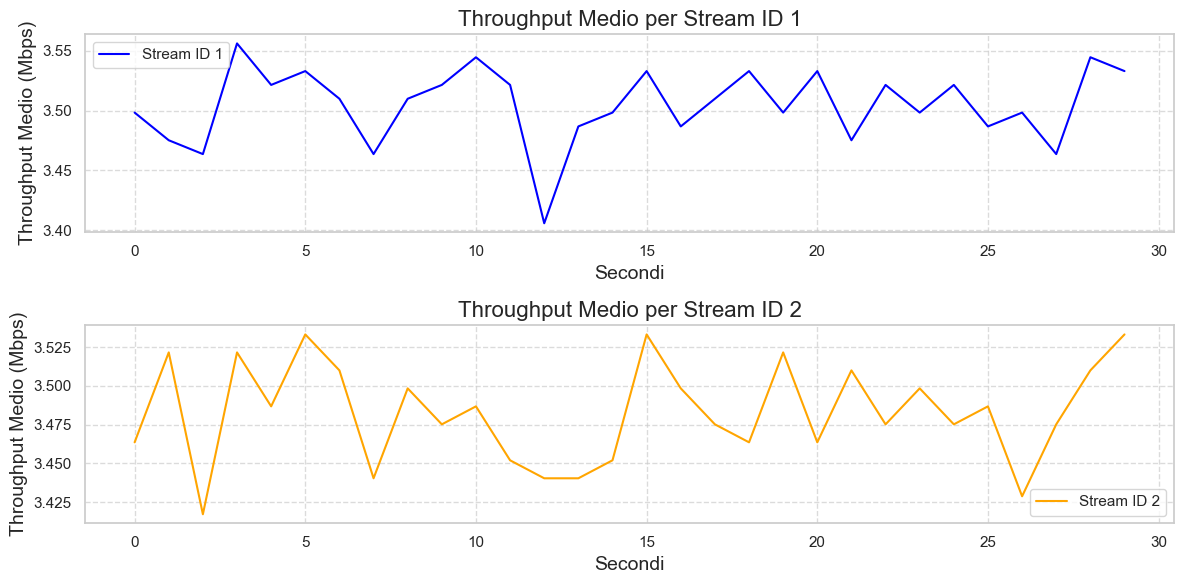
\includegraphics[width=1\textwidth]{t1_c0.png}
    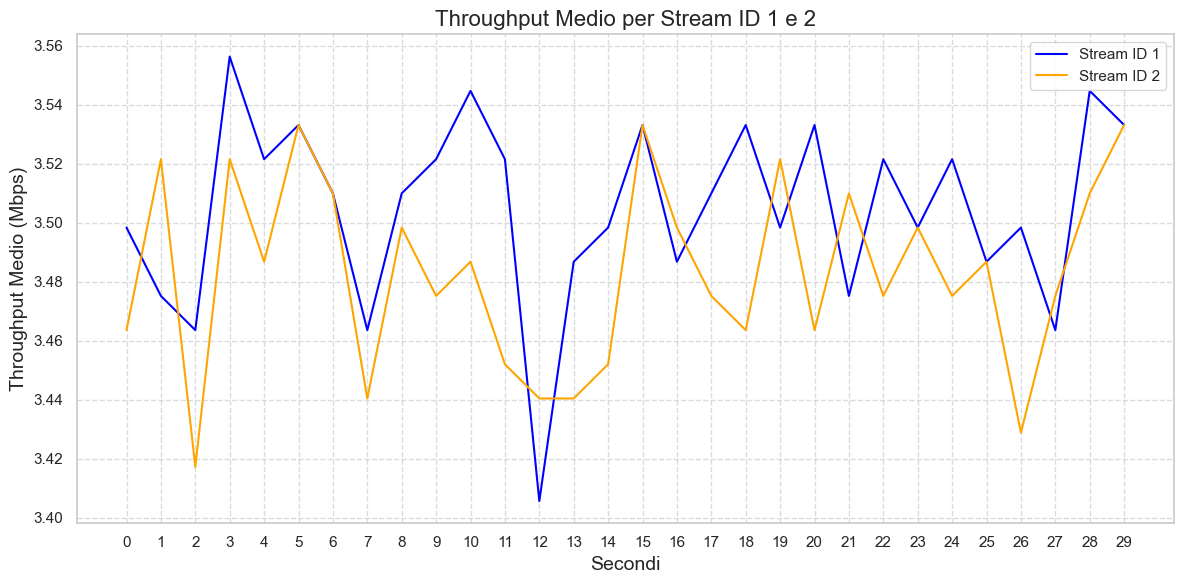
\includegraphics[width=1\textwidth]{t1_c0_main.png}
    \caption{QoS assente e congestione assente (Throughput medio)}
    \label{fig:t1_c0}
\end{figure}

\begin{figure}[h!]
    \centering
    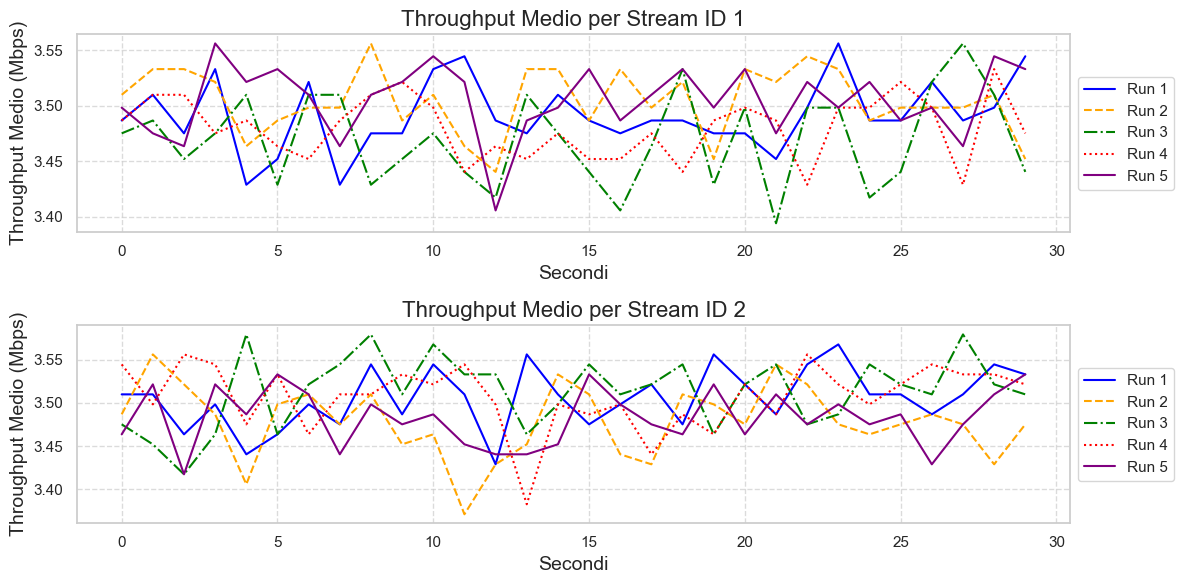
\includegraphics[width=1\textwidth]{t1_c0_ensemble.png}
    \caption{QoS assente e congestione assente (Grafico ensemble)}
    \label{fig:t1_c0_ensemble}
\end{figure}

\begin{figure}[h!]
    \centering
    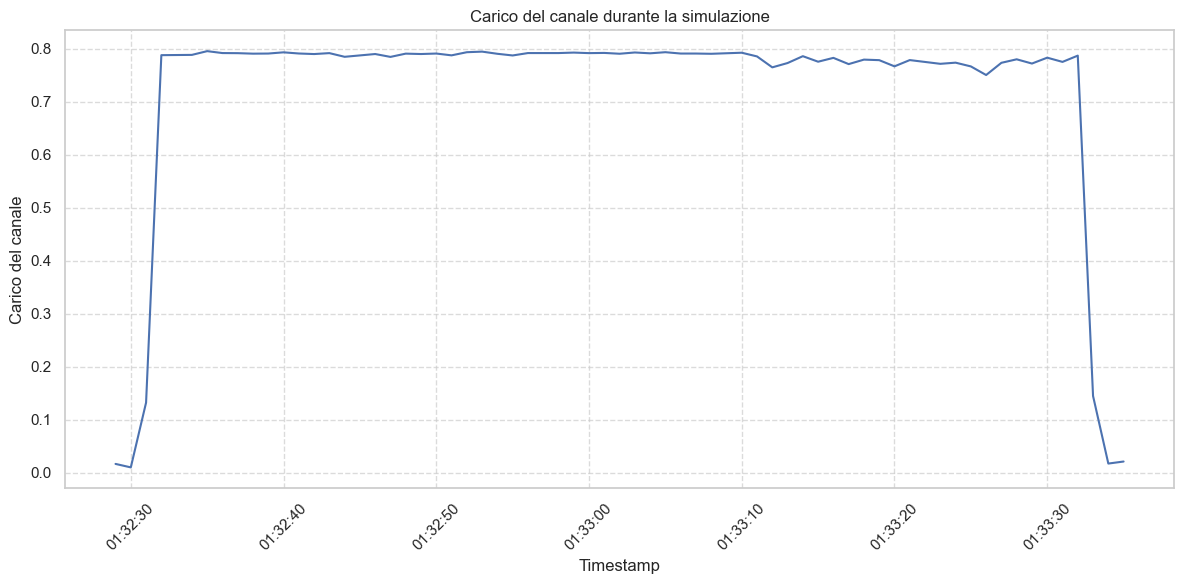
\includegraphics[width=1\textwidth]{t1_c0_load.png}
    \caption{QoS assente e congestione assente (Carico del canale)}
    \label{fig:t1_c0_load}
\end{figure}
\clearpage
\newpage
\subsection[QoS assente e congestione parziale]{QoS assente e congestione parziale}
L'assenza di politiche di \textit{QoS}, unito ad un canale parzialmente disturbato da CAM inviati dagli altri due dispositivi (Figura \ref{fig:t1_c1_load}), porta il throughput di ambedue i flussi ad essere simile ma inferiore rispetto al caso precedentemente discusso di circa il 10\%: 3.49 Mbps circa contro 3.13 Mbps qui (Tabella \ref{table:7} e Figure \ref{fig:t1_c1} e \ref{fig:t1_c1_ensemble}).

\begin{table}[h!]
    \centering
    \begin{tabular}{|>{\centering\arraybackslash}p{20em}|>{\centering\arraybackslash}p{7em}|} 
     \hline
     \textbf{} & \textbf{Valori} \\ 
     \hline
     \textbf{Throughput Medio per Stream ID 1} & 3.13 Mbps \\ 
     \hline
     \textbf{Throughput Medio per Stream ID 2} & 3.13 Mbps \\
     \hline
    \end{tabular}
    \caption{Valori medi caso \textit{QoS} assente e congestione parziale}
    \label{table:7}
\end{table}

\begin{figure}[h!]
    \centering
    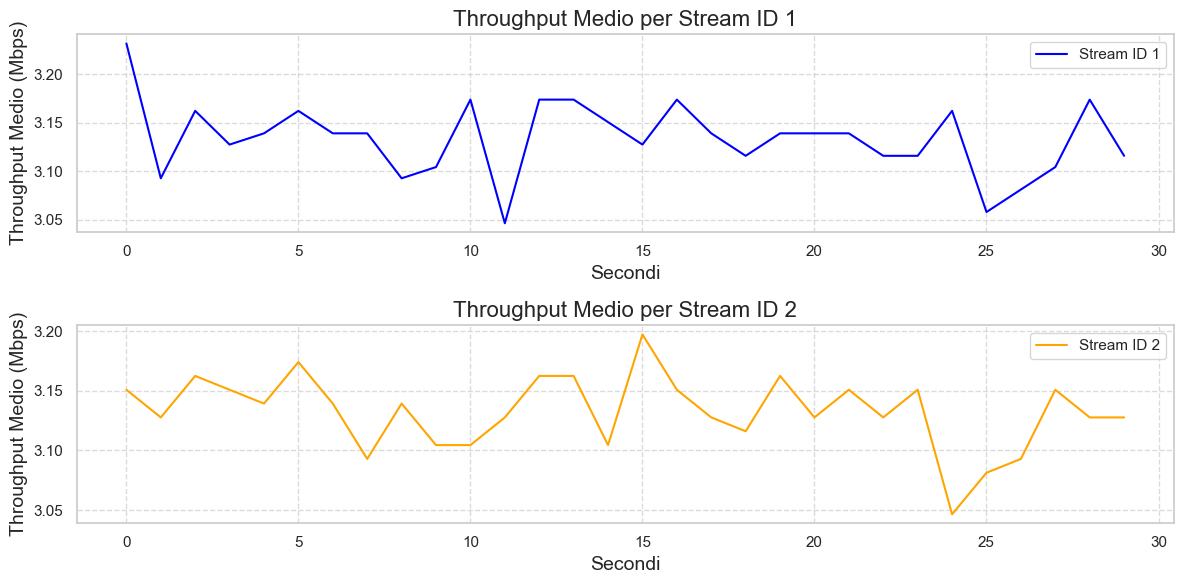
\includegraphics[width=1\textwidth]{t1_c1.png}
    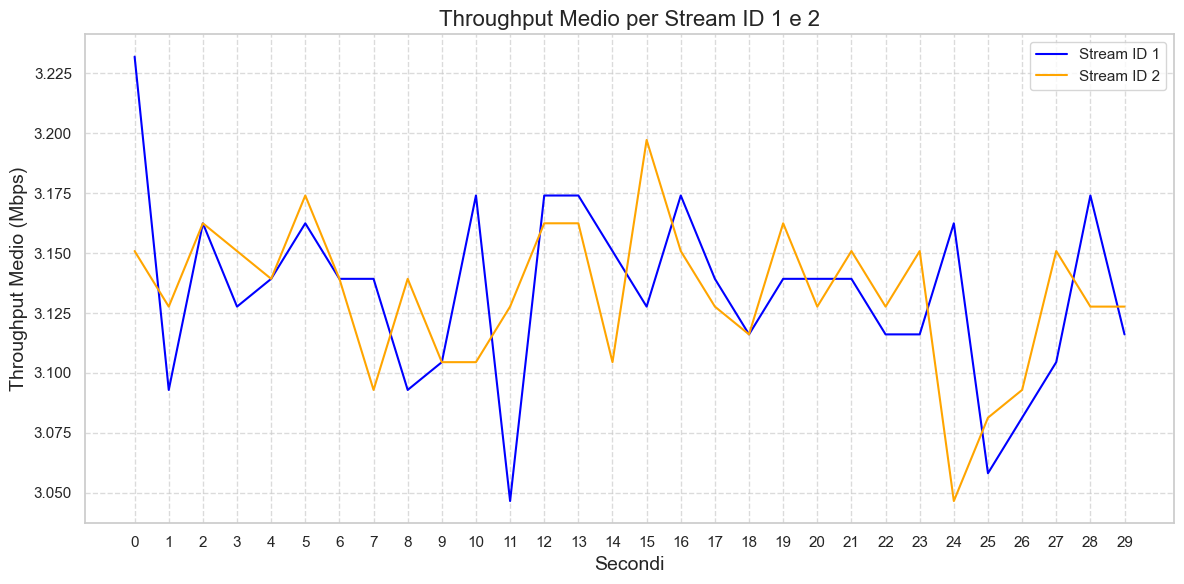
\includegraphics[width=1\textwidth]{t1_c1_main.png}
    \caption{QoS assente e congestione parziale (Throughput medio)}
    \label{fig:t1_c1}
\end{figure}

\begin{figure}[h!]
    \centering
    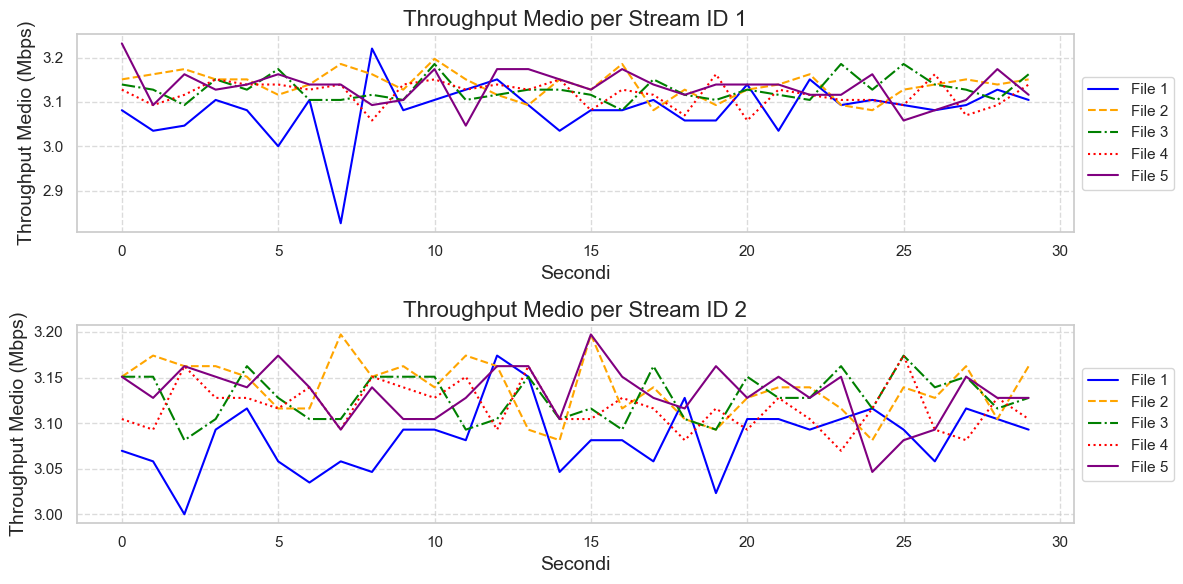
\includegraphics[width=1\textwidth]{t1_c1_ensemble.png}
    \caption{QoS assente e congestione parziale (Grafico ensemble)}
    \label{fig:t1_c1_ensemble}
\end{figure}

\begin{figure}[h!]
    \centering
    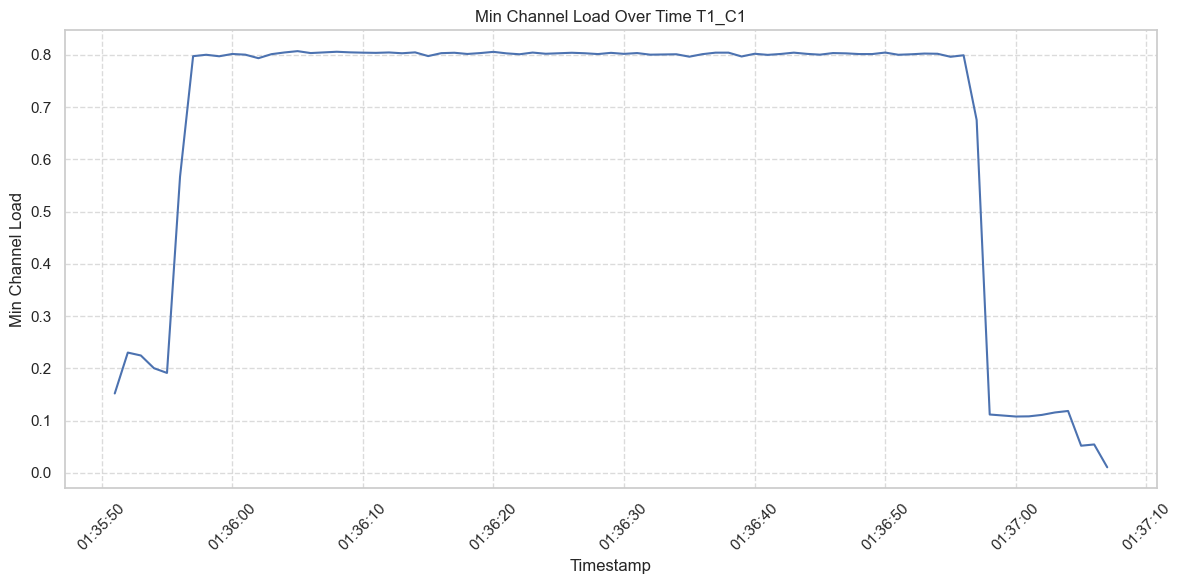
\includegraphics[width=1\textwidth]{t1_c1_load.png}
    \caption{QoS assente e congestione parziale (Carico del canale)}
    \label{fig:t1_c1_load}
\end{figure}
\clearpage
\newpage
\subsection[QoS assente e congestione totale]{QoS assente e congestione totale}
La completa saturazione del canale qui si fa sentire notevolmente (Figura \ref{fig:t1_c2_load}), in quanto il throughput di ambedue i flussi viene ridotto notevolmente con una minore propensione ad un valore stabile rispetto al caso senza congestione: 3.49 Mbps circa contro 1.14 Mbps circa qui (Tabella \ref{table:8} e Figure \ref{fig:t1_c2} e \ref{fig:t1_c2_ensemble}).
\begin{table}[h!]
    \centering
    \begin{tabular}{|>{\centering\arraybackslash}p{20em}|>{\centering\arraybackslash}p{7em}|} 
     \hline
     \textbf{} & \textbf{Valori} \\ 
     \hline
     \textbf{Throughput Medio per Stream ID 1} & 1.14 Mbps \\ 
     \hline
     \textbf{Throughput Medio per Stream ID 2} & 1.19 Mbps \\
     \hline
    \end{tabular}
    \caption{Valori medi caso \textit{QoS} assente e congestione totale}
    \label{table:8}
\end{table}

\begin{figure}[h!]
    \centering
    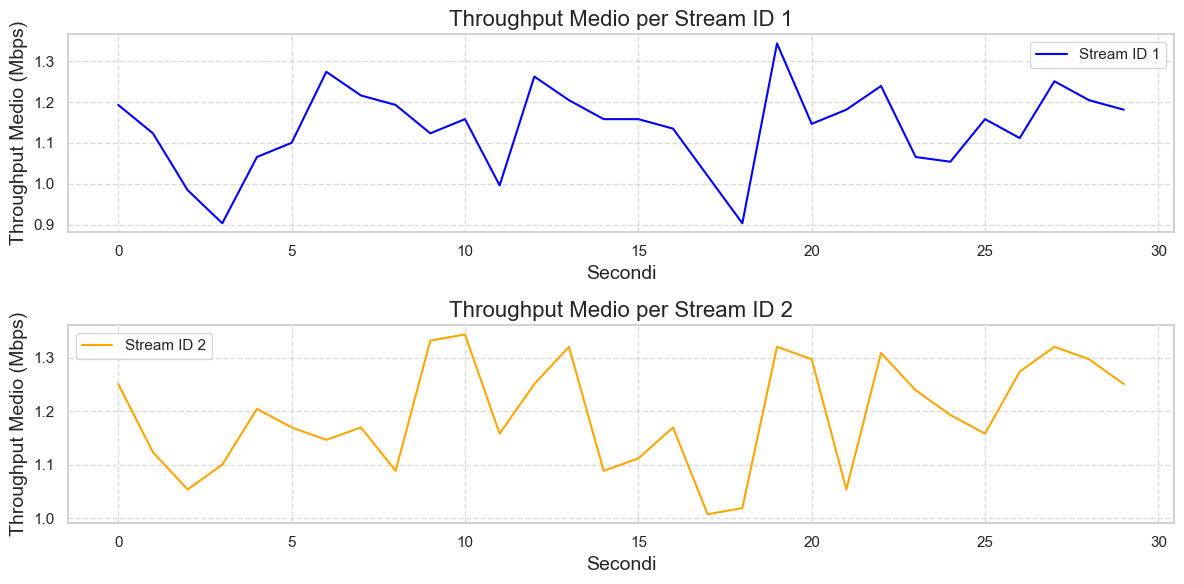
\includegraphics[width=1\textwidth]{t1_c2.png}
    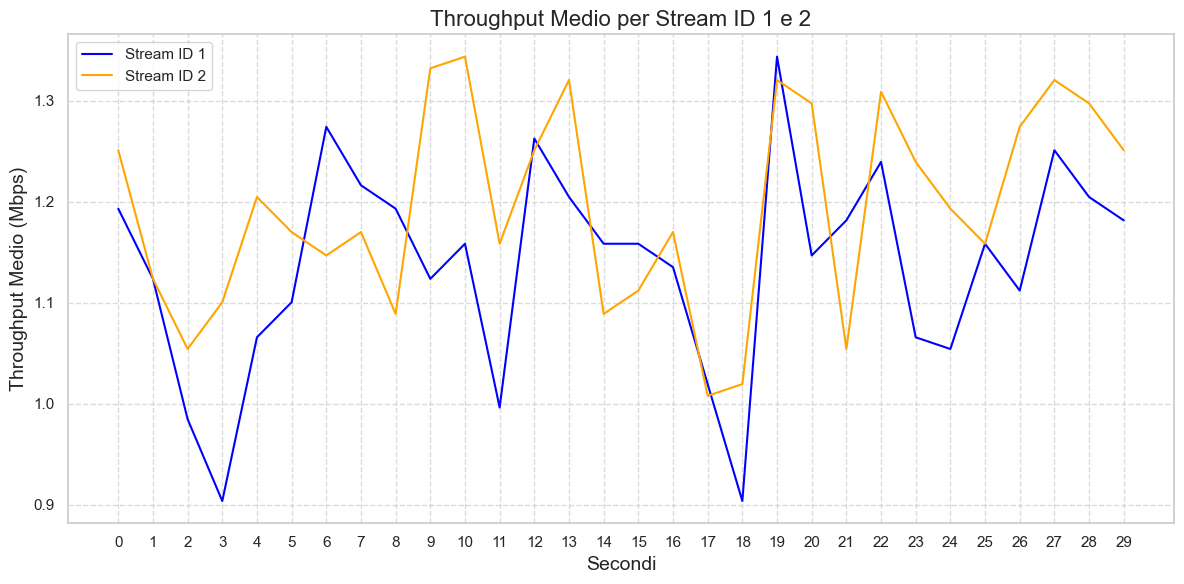
\includegraphics[width=1\textwidth]{t1_c2_main.png}
    \caption{QoS assente e congestione totale (Throughput medio)}
    \label{fig:t1_c2}
\end{figure}

\begin{figure}[h!]
    \centering
    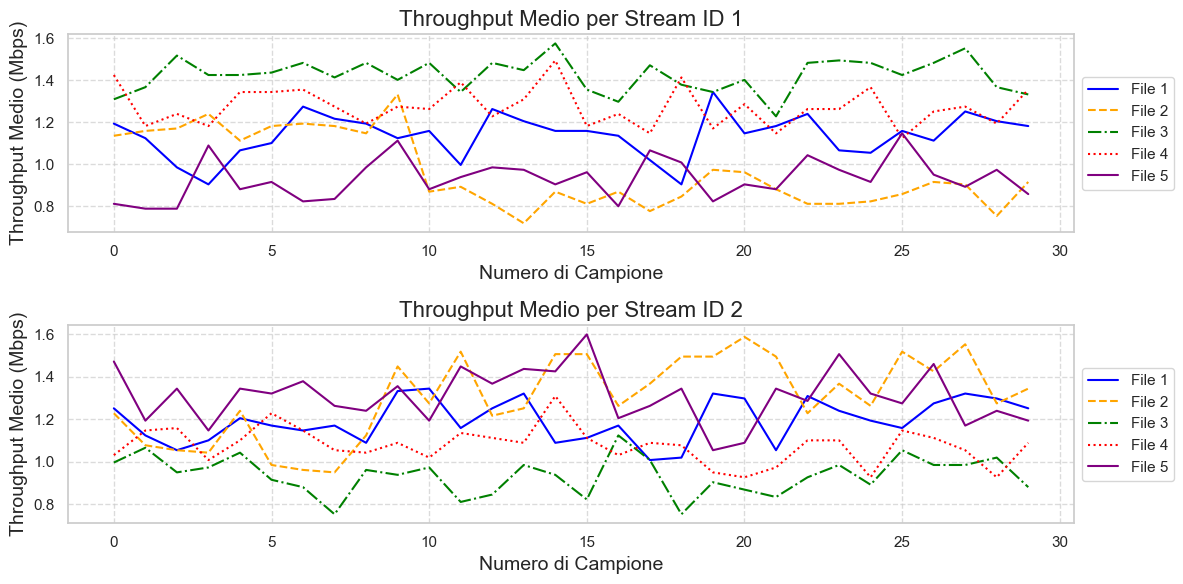
\includegraphics[width=1\textwidth]{t1_c2_ensemble.png}
    \caption{QoS assente e congestione totale (Grafico ensemble)}
    \label{fig:t1_c2_ensemble}
\end{figure}

\begin{figure}[h!]
    \centering
    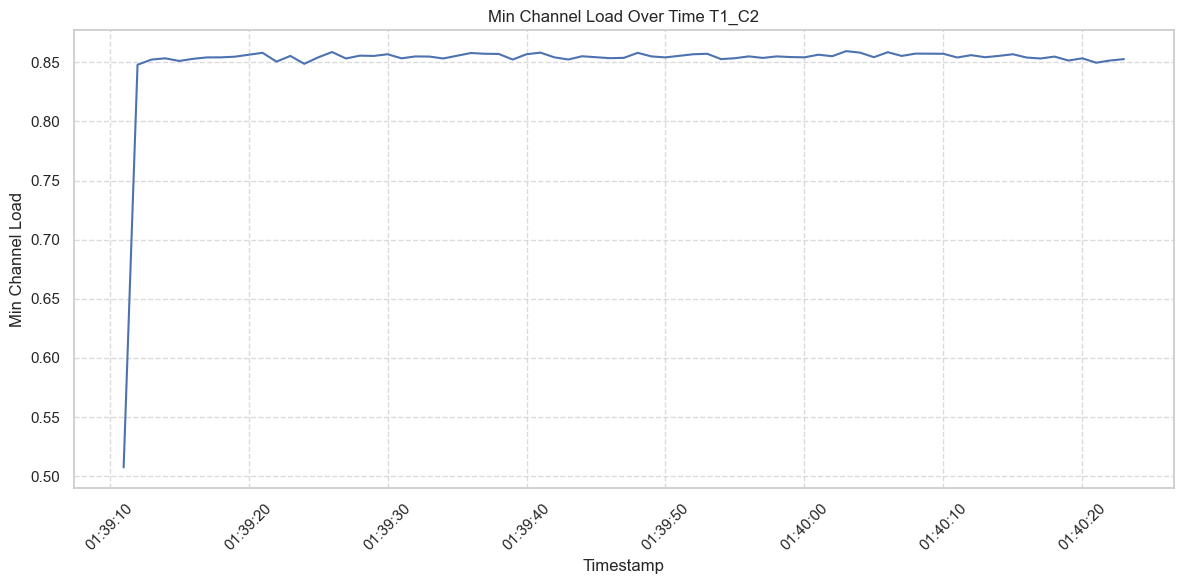
\includegraphics[width=1\textwidth]{t1_c2_load.png}
    \caption{QoS assente e congestione totale (Carico del canale)}
    \label{fig:t1_c2_load}
\end{figure}
\clearpage
\newpage
\subsection[QoS presente e congestione assente]{QoS presente e congestione assente}
L'inserimento, qui, di politiche di \textit{QoS}, unito ad un canale quasi completamente vuoto e libero da trasmissioni (Figura \ref{fig:t2_c0_load}), porta il throughput del flusso a priorità maggiore ad sopraffare completamente l'altro a priorità minore (Tabella \ref{table:9} e Figure \ref{fig:t2_c0} e \ref{fig:t2_c0_ensemble}). Salta, inoltre, palesemente all'occhio che la somma dei throughput dei flussi è maggiore rispetto al medesimo caso di congestione senza però l'applicazione di politiche di \textit{QoS} (8.57 Mbps vs 7.00 Mbps circa).

\begin{table}[h!]
    \centering
    \begin{tabular}{|>{\centering\arraybackslash}p{20em}|>{\centering\arraybackslash}p{7em}|} 
     \hline
     \textbf{} & \textbf{Valori} \\ 
     \hline
     \textbf{Throughput Medio per Stream ID 1} & 7.96 Mbps \\ 
     \hline
     \textbf{Throughput Medio per Stream ID 2} & 0.61 Mbps \\
     \hline
    \end{tabular}
    \caption{Valori medi caso \textit{QoS} presente e congestione assente}
    \label{table:9}
\end{table}

\begin{figure}[h!]
    \centering
    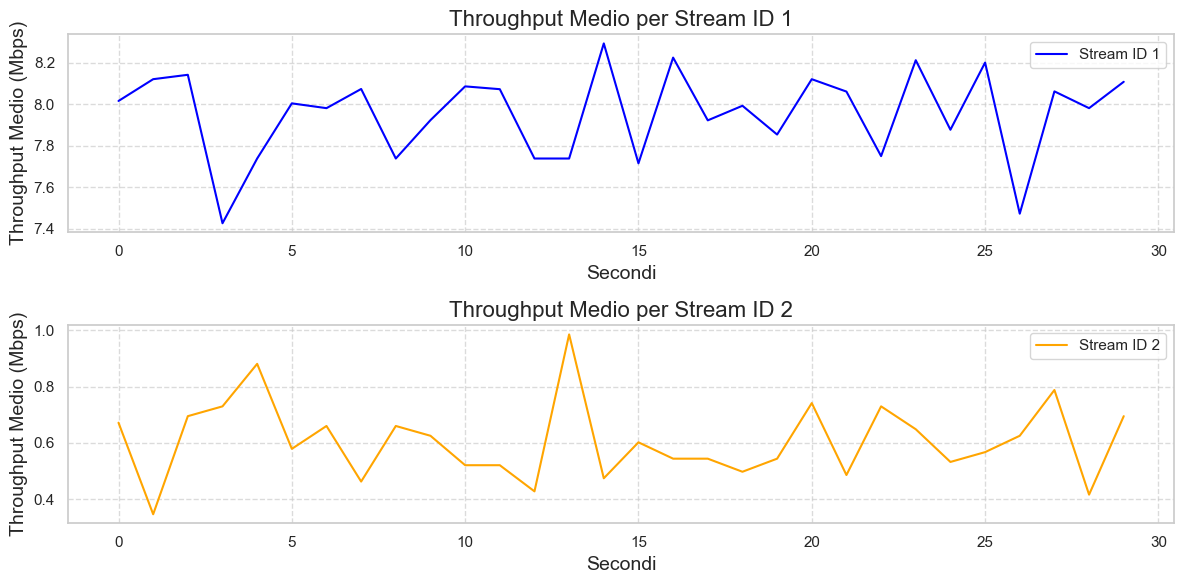
\includegraphics[width=0.9\textwidth]{t2_c0.png}
    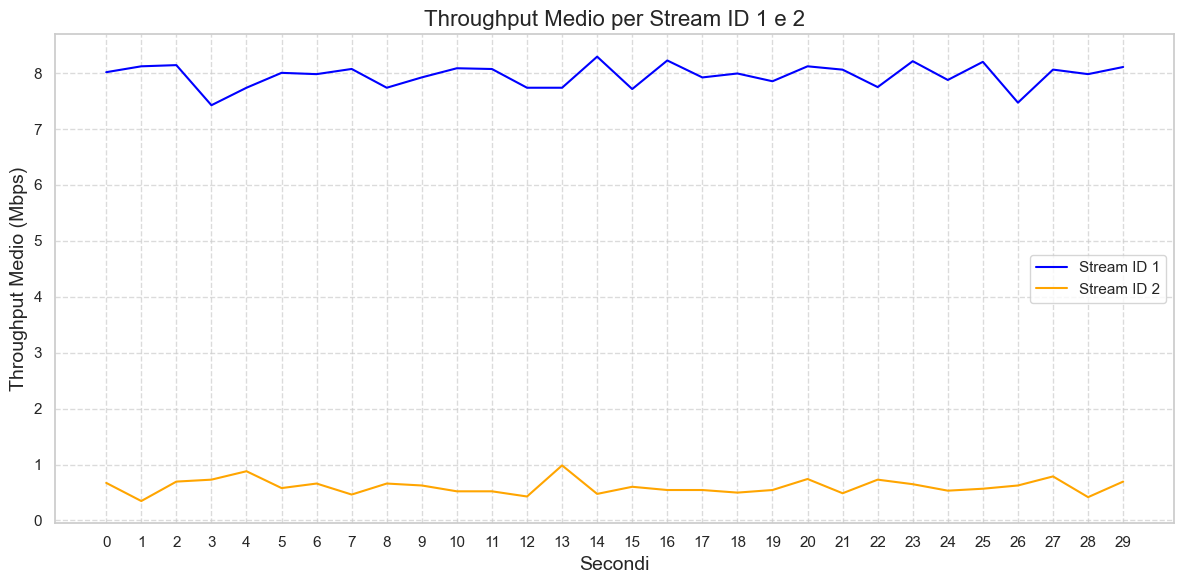
\includegraphics[width=0.9\textwidth]{t2_c0_main.png}
    \caption{QoS presente e congestione assente (Throughput medio)}
    \label{fig:t2_c0}
\end{figure}

\begin{figure}[h!]
    \centering
    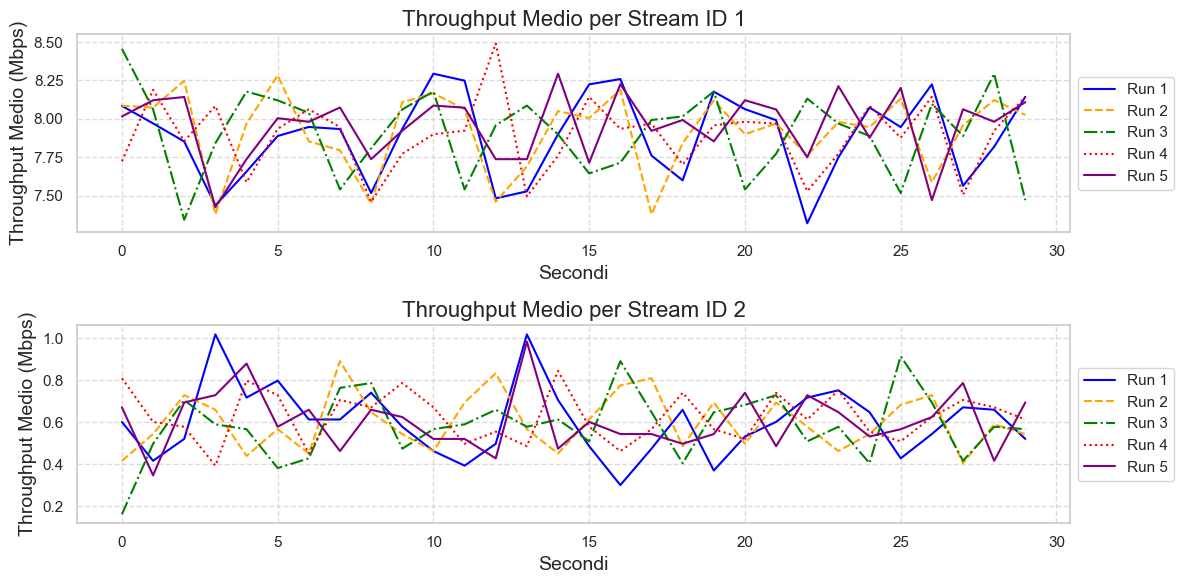
\includegraphics[width=1\textwidth]{t2_c0_ensemble.png}
    \caption{QoS presente e congestione assente (Grafico ensemble)}
    \label{fig:t2_c0_ensemble}
\end{figure}

\begin{figure}[h!]
    \centering
    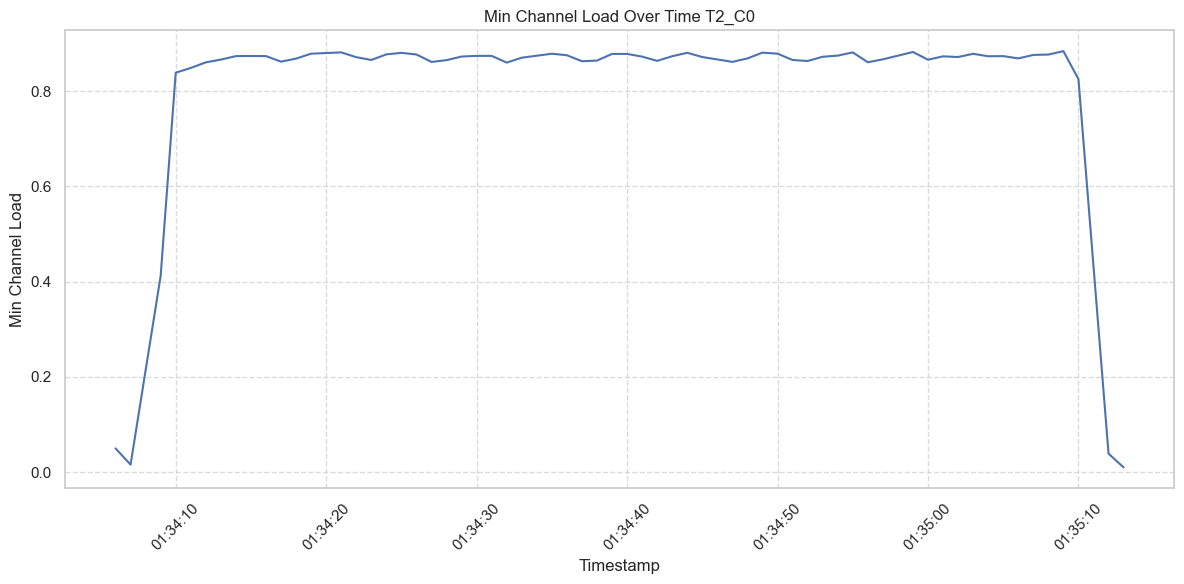
\includegraphics[width=1\textwidth]{t2_c0_load.png}
    \caption{QoS presente e congestione assente (Carico del canale)}
    \label{fig:t2_c0_load}
\end{figure}
\clearpage
\newpage
\subsection[QoS presente e congestione parziale]{QoS presente e congestione parziale}
In questa situazione, si osserva che il throughput fatica a stabilizzarsi, sia per il flusso a priorità maggiore che per l'altro flusso. Ci vuole un tempo considerevole affinché il throughput raggiunga un valore stabile. Il flusso VO inizia con una velocità di circa 6 Mbps e tende ad aumentare, a discapito dell'altro flusso, che parte da circa 1.2 Mbps e rallenta fino a scendere a 0.4 Mbps. Palese anche qui un throughput maggiore rispetto al caso senza \textit{QoS} (7.50 Mbps vs 6.00 Mbps circa).

Il valore di throughput medio è ovviamente influenzato dal comportamento appena descritto.

\begin{table}[h!]
    \centering
    \begin{tabular}{|>{\centering\arraybackslash}p{20em}|>{\centering\arraybackslash}p{7em}|} 
     \hline
     \textbf{} & \textbf{Valori} \\ 
     \hline
     \textbf{Throughput Medio per Stream ID 1} & 6.73 Mbps \\ 
     \hline
     \textbf{Throughput Medio per Stream ID 2} & 0.77 Mbps \\
     \hline
    \end{tabular}
    \caption{Valori medi caso \textit{QoS} presente e congestione parziale}
    \label{table:10}
\end{table}

\begin{figure}[h!]
    \centering
    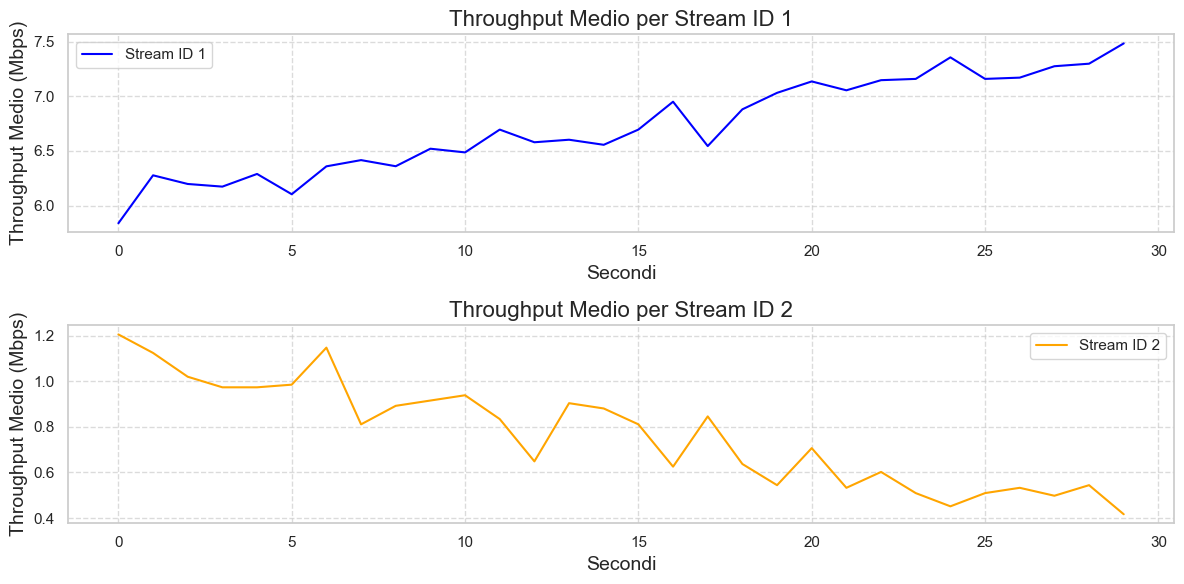
\includegraphics[width=0.9\textwidth]{t2_c1.png}
    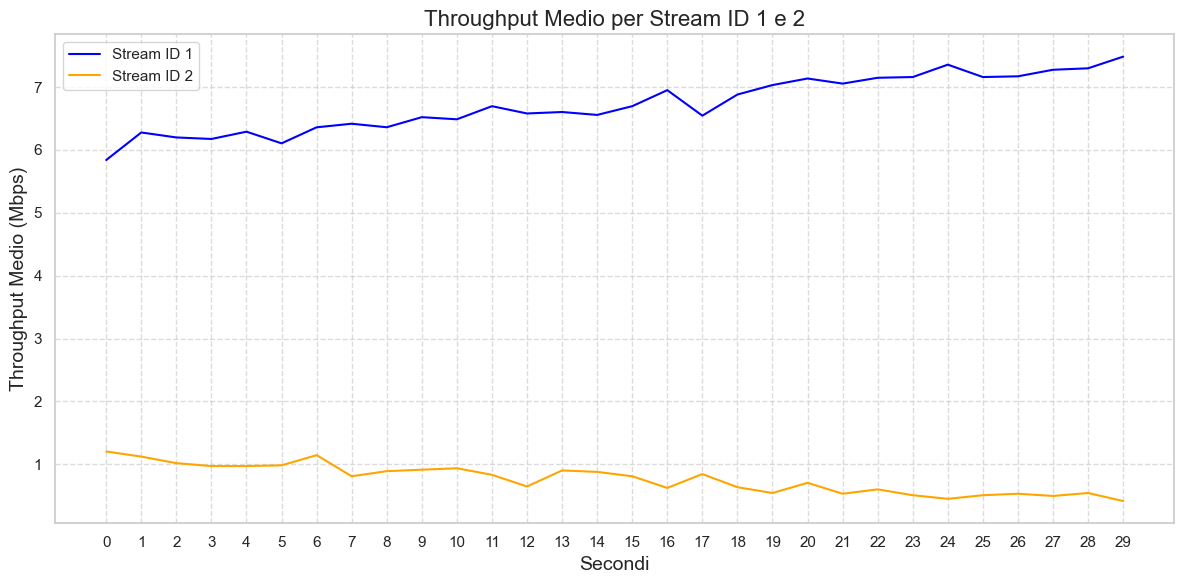
\includegraphics[width=0.8\textwidth]{t2_c1_main.png}
    \caption{QoS presente e congestione parziale (Throughput medio)}
    \label{fig:t2_c1}
\end{figure}

\begin{figure}[h!]
    \centering
    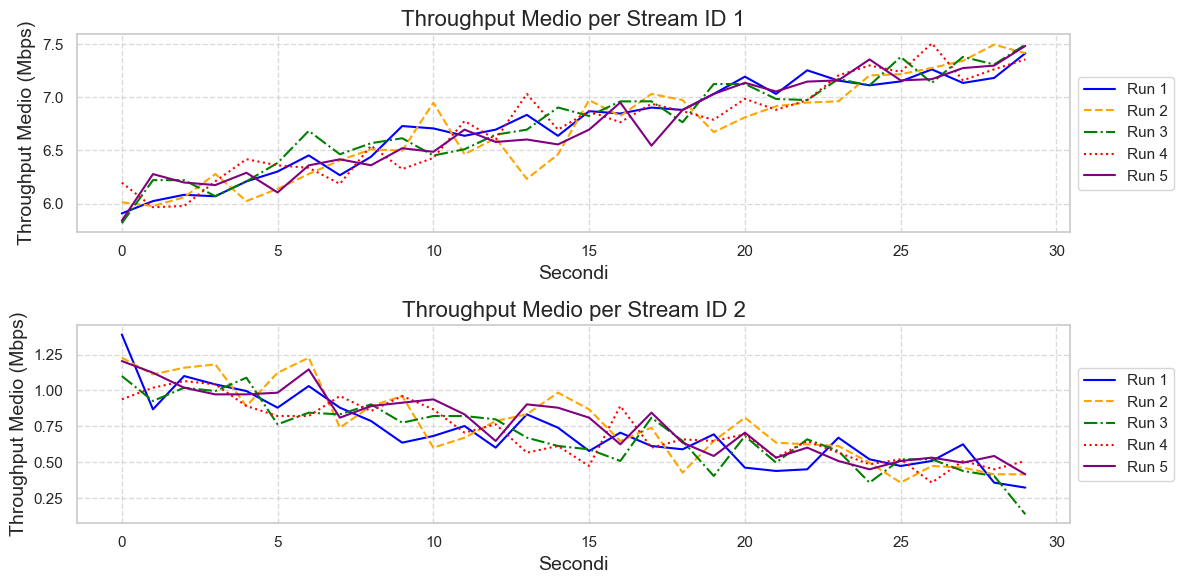
\includegraphics[width=1\textwidth]{t2_c1_ensemble.png}
    \caption{QoS presente e congestione parziale (Grafico ensemble)}
    \label{fig:t2_c1_ensemble}
\end{figure}

\begin{figure}[h!]
    \centering
    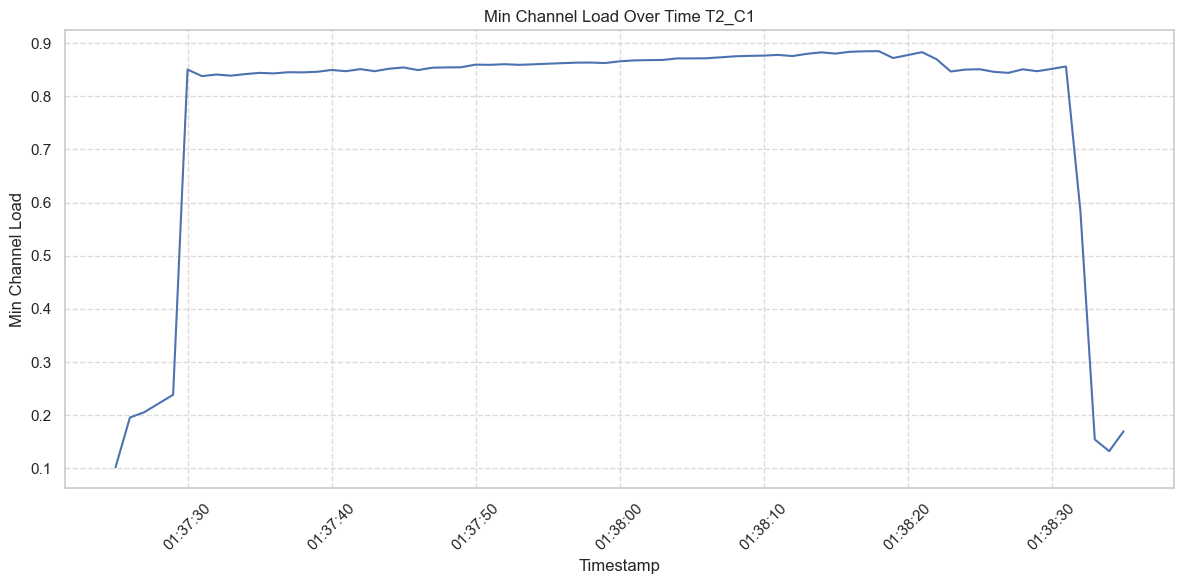
\includegraphics[width=1\textwidth]{t2_c1_load.png}
    \caption{QoS presente e congestione parziale (Carico del canale)}
    \label{fig:t2_c1_load}
\end{figure}
\clearpage
\newpage
\subsection[QoS presente e congestione totale]{QoS presente e congestione totale}
La completa saturazione del canale qui si fa sentire notevolmente (Figura \ref{fig:t2_c2_load}), in quanto il throughput di ambedue i flussi viene ridotto notevolmente con un inoltre minore propensione ad essere stabile rispetto al caso senza congestione. (Tabella \ref{table:11} e Figure \ref{fig:t2_c2} e \ref{fig:t2_c2_ensemble}). L'applicazione di politiche di \textit{QoS} porta, naturalmente, ad un throughput medio maggiore del flusso a priorità maggiore.

Cosa molto importante qui è il throughput totale raggiunto rispetto al caso senza code di priorità, ma questo verrà discusso a breve.

\begin{table}[h!]
    \centering
    \begin{tabular}{|>{\centering\arraybackslash}p{20em}|>{\centering\arraybackslash}p{7em}|} 
     \hline
     \textbf{} & \textbf{Valori} \\ 
     \hline
     \textbf{Throughput Medio per Stream ID 1} & 6.19 Mbps \\ 
     \hline
     \textbf{Throughput Medio per Stream ID 2} & 0.30 Mbps \\
     \hline
    \end{tabular}
    \caption{Valori medi caso \textit{QoS} presente e congestione totale}
    \label{table:11}
\end{table}

\begin{figure}[h!]
    \centering
    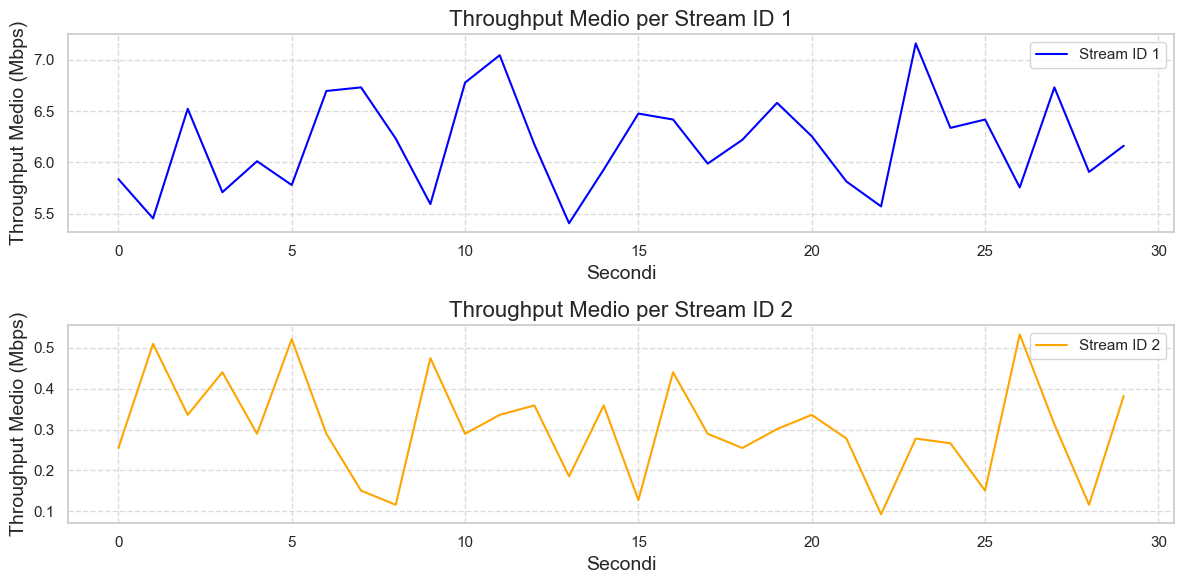
\includegraphics[width=0.9\textwidth]{t2_c2.png}
    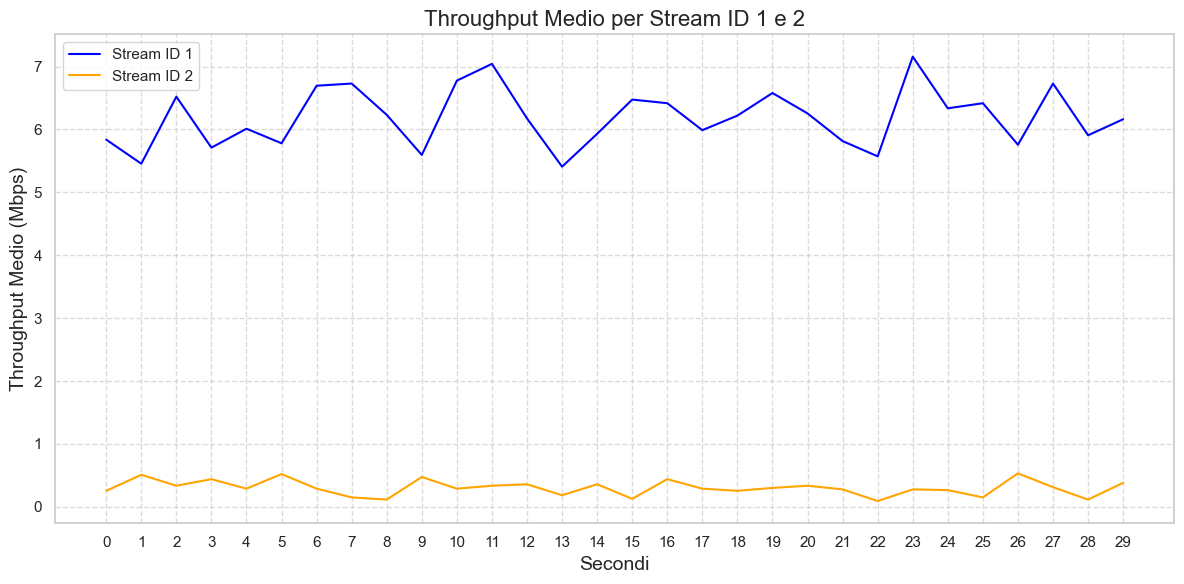
\includegraphics[width=0.9\textwidth]{t2_c2_main.png}
    \caption{QoS presente e congestione totale (Throughput medio)}
    \label{fig:t2_c2}
\end{figure}

\begin{figure}[h!]
    \centering
    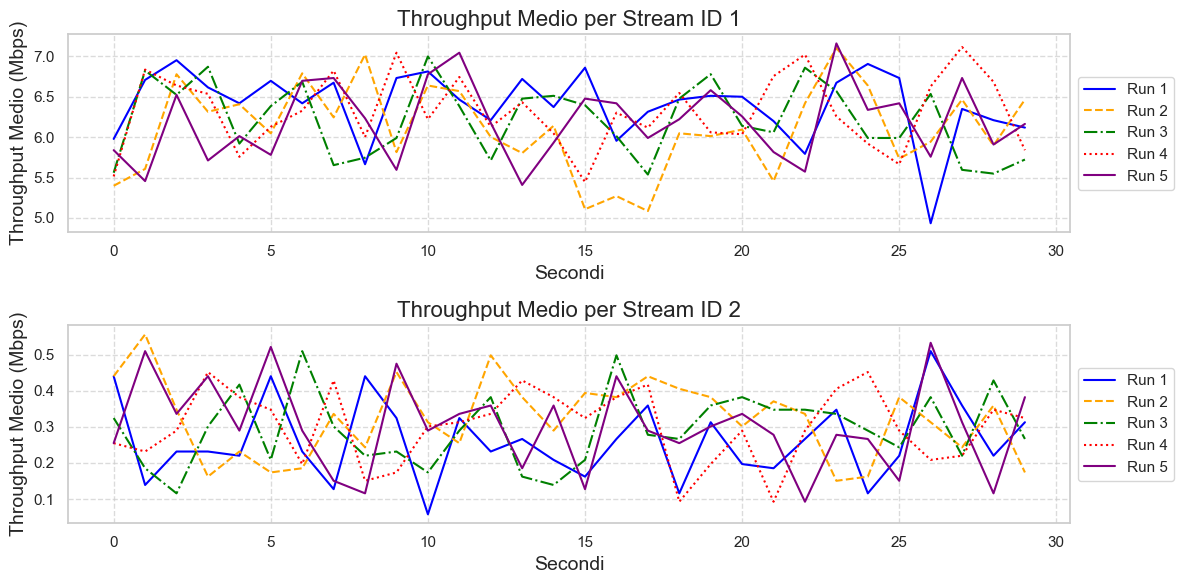
\includegraphics[width=1\textwidth]{t2_c2_ensemble.png}
    \caption{QoS presente e congestione totale (Grafico ensemble)}
    \label{fig:t2_c2_ensemble}
\end{figure}

\begin{figure}[h!]
    \centering
    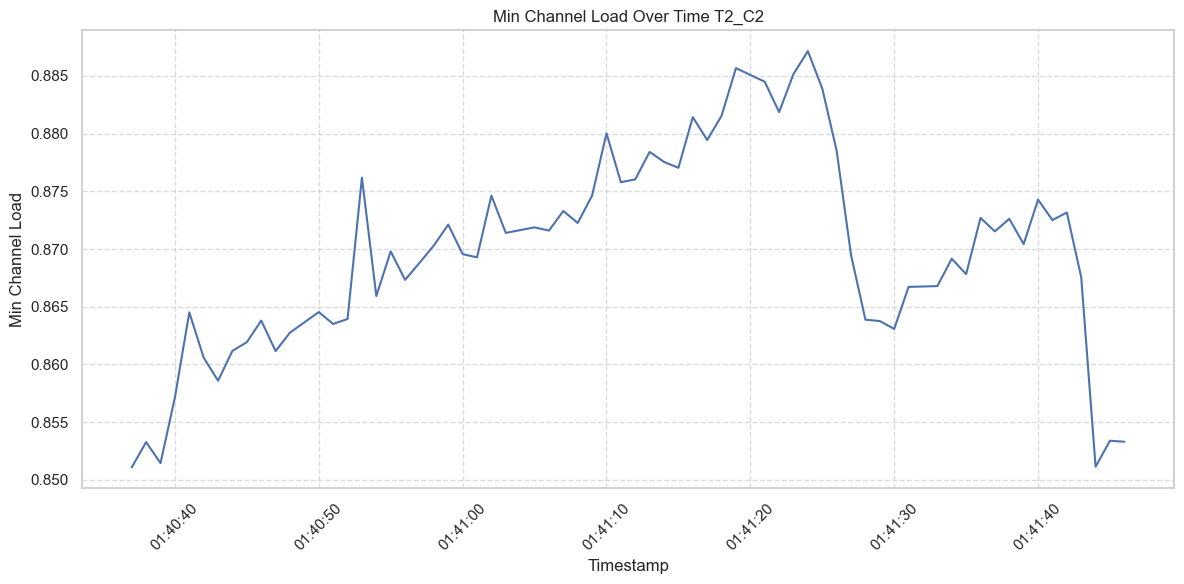
\includegraphics[width=1\textwidth]{t2_c2_load.png}
    \caption{QoS presente e congestione totale (Carico del canale)}
    \label{fig:t2_c2_load}
\end{figure}
\clearpage
\newpage
\subsection[Analisi dei risultati]{Analisi dei risultati}
Dai dati raccolti e presentati nelle sezioni precedenti, riportati tutti insieme per comodità in Tabella \ref{table:12} (nei casi in cui sono state applicate politiche di \textit{QoS}, lo \textbf{Stream 1} è quello con priorità \textit{AC\_VO}, mentre lo \textbf{Stream 2} è quello con priorità \textit{AC\_BK}), è evidente che la presenza di disturbi, anche se moderati, influisce sulla trasmissione dei due flussi TCP dal nodo server al nodo client. Si osserva, con l'aumento della congestione del canale, la transizione da un throughput elevato e relativamente stabile a prestazioni via via più basse, con una tendenza della velocità media a diventare meno stabile e più soggetta a oscillazioni.

\begin{table}[h!]
    \centering
    \begin{tabular}{|p{20em}|>{\centering\arraybackslash}p{5em}|>{\centering\arraybackslash}p{5em}|} 
     \hline
     \textbf{Caso} & \textbf{Valori} & \textbf{Varianza}\\ 
     \hline
     \textbf{QoS assente e congestione assente (Stream 1)} & 3.49 & 0.000972\\ 
     \hline
     \textbf{QoS assente e congestione assente (Stream 2)} & 3.47 & 0.000972 \\
     \hline
     \textbf{QoS assente e congestione parziale (Stream 1)} & 3.13 & 0.00144\\ 
     \hline
     \textbf{QoS assente e congestione parziale (Stream 2)} & 3.13 & 0.00092\\
     \hline
     \textbf{QoS assente e congestione totale (Stream 1)} & 1.14 & 0.0919\\ 
     \hline
     \textbf{QoS assente e congestione totale (Stream 2)} & 1.19 & 0.01540\\
     \hline
     \textbf{QoS presente e congestione assente (Stream 1)} & 7.96 & 0.04425\\ 
     \hline
     \textbf{QoS presente e congestione assente (Stream 2)} & 0.61 & 0.01867\\
     \hline
     \textbf{QoS presente e congestione parziale (Stream 1)} & 6.73 & 0.1835\\ 
     \hline
     \textbf{QoS presente e congestione parziale (Stream 2)} & 0.77 & 0.04963\\
     \hline
     \textbf{QoS presente e congestione totale (Stream 1)} & 6.19 & 0.20920\\ 
     \hline
     \textbf{QoS presente e congestione totale (Stream 2)} & 0.30 & 0.01466\\
     \hline
    \end{tabular}
    \caption{Confronto risultati (Valori in Mbps)}
    \label{table:12}
\end{table}

Questa situazione si verifica sia in assenza di politiche di \textit{QoS}, sia quando si assegna una priorità maggiore a uno dei flussi rispetto all'altro. In entrambe le circostanze, i valori di throughput medio risultano generalmente meno stabili e caratterizzati da oscillazioni temporali; la variabilità tende a aumentare in tutti i casi di congestione. 

Inoltre, applicando le priorità, si può notare un cambiamento nel tempo necessario affinché ciascun flusso raggiunga un valore di velocità di throughput su cui si stabilizzerà (anche per via delle politiche di controllo della congestione attuate \textit{under-the-hood} dal protocollo TCP):
\begin{itemize}
    \item \textit{Nessuna congestione}: il throughput di VO raggiunge immediatamente il valore massimo ed è apparentemente stabile, grazie a un canale libero che consente ad esso di trasmettere al massimo, mentre il flusso BK utilizza la banda rimanente.
    \item \textit{Congestione parziale}: il throughput di VO ha una tendenza monotòna crescente, ma molto lenta a causa dei disturbi nel canale, che impediscono un rapido raggiungimento della massima velocità possibile; ovviamente ne risente anche il flusso BK.
    \item \textit{Piena congestione}: il throughput di ambedue i flussi rimane basso a causa della super congestione del canale.
\end{itemize}

\noindent Questo comportamento non viene riscontrato nel caso in cui non siano state applicate classi di servizio specifiche.

\begin{figure}[h!]
    \centering
    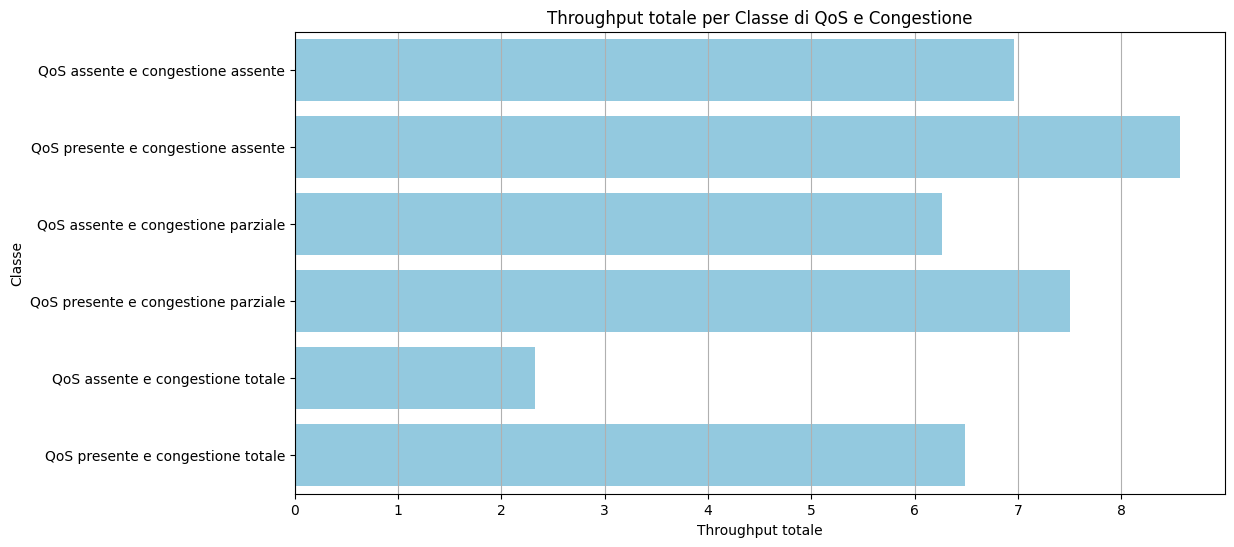
\includegraphics[width=1\textwidth]{throughput_bar.png}
    \caption{Throughput totale per Classe di QoS e Congestione}
    \label{fig:throughput_bar}
\end{figure}

Volendosi focalizzare, ora, sui valori totali di throughput medio (Figura \ref{fig:throughput_bar}), si osserva che, in assenza di \textit{QoS} e in condizioni di congestione assente, la somma delle velocità dei flussi è pari a circa 6.96 Mbps. Questo valore, sebbene relativamente elevato, indica che, in condizioni ottimali, per un canale di trasmissione con throughput teorico massimo di 10 Mbps teorici, la trasmissione può operare in modo efficace. Tuttavia, l'introduzione della congestione comporta una diminuzione della somma, che scende a 6.26 Mbps in condizioni di congestione parziale e a 2.33 Mbps in condizioni di congestione totale. Tale calo significativo evidenzia come apparentemente l'assenza di politiche di priorità renda i flussi vulnerabili agli effetti negativi della congestione, portando a una degradazione delle performance.

Al contrario, quando la \textit{QoS} è presente, la somma delle velocità dei flussi presenta un comportamento nettamente diverso. In condizioni di congestione assente, la somma raggiunge 8.57 Mbps, rappresentando un incremento significativo rispetto alla somma riscontrata in assenza di \textit{QoS}. Questo risultato suggerisce che l'implementazione delle classi di priorità consente ai flussi di operare in maniera più efficiente, ottimizzando l'utilizzo della banda disponibile. Anche in condizioni di congestione parziale, la somma dei flussi rimane elevata, attestandosi a 7.50 Mbps. Tale risultato è particolarmente rilevante, in quanto indica che la \textit{QoS} è in grado di mantenere buone performance anche in situazioni che normalmente potrebbero compromettere la qualità del servizio.

Infine, anche in condizioni di congestione totale, la somma dei flussi con \textit{QoS} presente è pari a 6.49 Mpbs, un valore notevolmente superiore rispetto al corrispondente 2.33 Mbps osservato in assenza di priorità. Questo dato mette ulteriormente in evidenza l'importanza di quest'ultima nella mitigazione degli effetti negativi della congestione.

In conclusione, l'analisi dei dati relativi al throughput dei flussi TCP in presenza e assenza di \textit{Quality of Service (QoS)} enfatizza l'importanza di politiche di gestione del traffico, specialmente in scenari di congestione. I risultati mostrano chiaramente che l'implementazione di essa, dando maggiore priorità ad un flusso piuttosto che ad un altro, consente di mantenere performance più elevate e stabili, anche in condizioni avverse. Inoltre, la somma dei valori di throughput dei flussi, ovvero il throughput totale del canale, che varia significativamente in base alla presenza di \textit{QoS} e al livello di congestione, sottolinea ancora di più come la capacità di gestire il traffico dati possa influenzare direttamente l'efficacia della trasmissione.

Questi principi sono particolarmente rilevanti in contesti applicativi ad alta intensità di dati, come nel caso della guida di veicoli da remoto. Sebbene non sia l'unico ambito in cui la \textit{QoS} gioca un ruolo cruciale, la necessità di garantire una comunicazione affidabile e tempestiva è fondamentale in qualsiasi applicazione che richieda un'interazione in tempo reale. La capacità di mantenere un throughput elevato e una latenza ridotta è essenziale non solo per garantire la sicurezza e l'affidabilità delle operazioni, ma anche per migliorare l'esperienza complessiva dell'utente. Inoltre, è importante notare che le velocità di trasmissione raggiunte, persino nelle condizioni peggiori, sono superiori a quanto effettivamente necessario per le applicazioni specifiche. Questo surplus di capacità non solo offre un margine di sicurezza contro eventuali fluttuazioni nel traffico di rete, ma consente anche di gestire situazioni impreviste, come picchi di richiesta o congestione temporanea.

In sintesi, l'adozione di meccanismi di \textit{QoS} si rivela indispensabile per affrontare le sfide legate alla congestione e per ottimizzare le performance di rete, particolarmente in un contesto \textit{safety critical} come quello delle VANET.